\begin{tikzpicture}
\node[anchor=south west,inner sep=0] at (0,0) {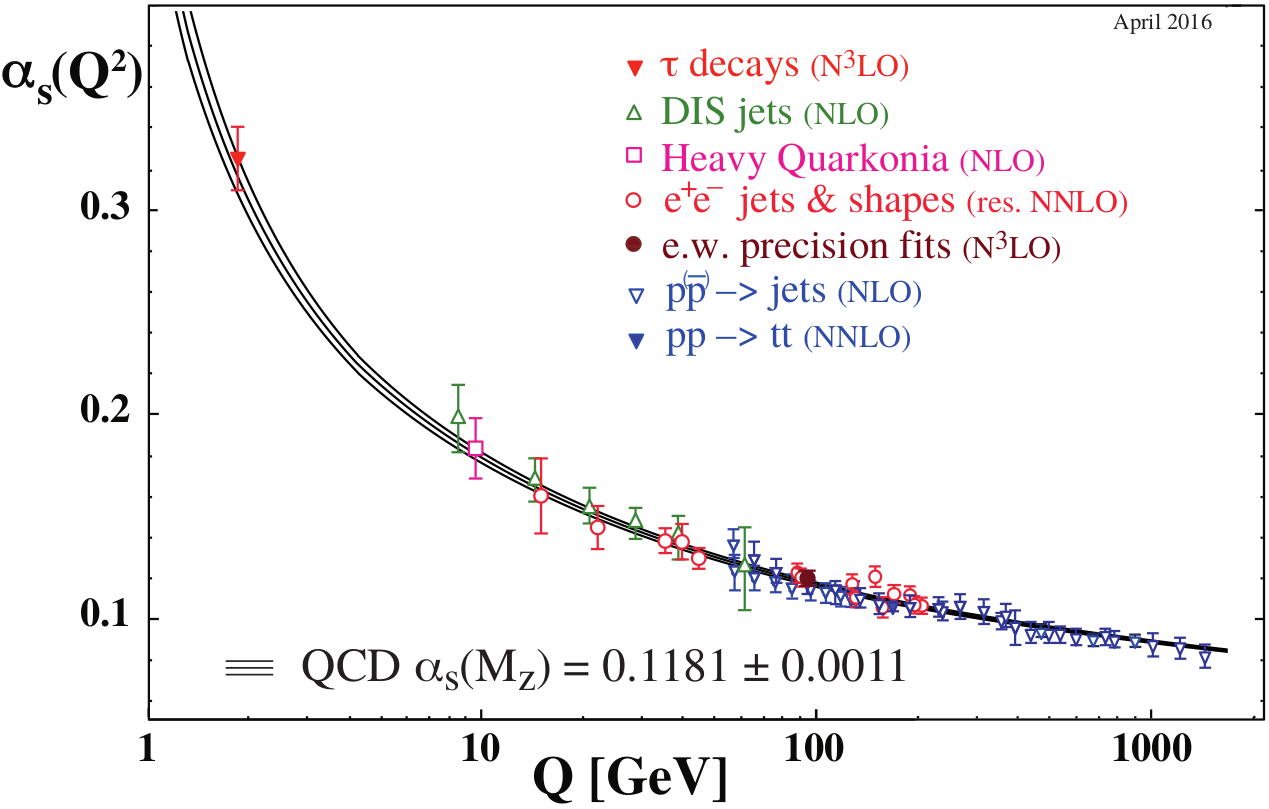
\includegraphics[width=8cm]{\PhDthesisdir/plots_and_images/from_PDG_booklet_2020/QCD_value_fct_Q.png}};

% masks
\fill [white] (0,0) rectangle (1.36,8.24);
\fill [white] (0,0) rectangle (8,0.96);
\fill [white] (1.6,1.2) rectangle (5.6,1.68);

% X axis
\foreach \val in {1,10,100,1000}{
\draw ({1.4+(7.32-1.4)*ln(\val)/ln(1000)}, 0.68) node {\footnotesize \num{\val}\vphantom{ÀQg}};
}
\draw (4.8, .2) node {\normalsize $k$ (\SI{}{\GeV})};

% Y axis
\foreach \val in {0.05,0.10,0.15,0.20,0.25,0.30,0.35}{
\draw (1.4, {1+(\val-0.05)/(0.35-0.05)*(8.1-1)}) node [left] {\footnotesize \num{\val}};
}

\draw (.4,4.64) node [rotate=90] {\normalsize $\alpha_s(k)$} ;


\draw (1.68, 1.44) node [right] {\small $\equiv$ QCD $\alpha_s(m_{\Zboson}) = \num{0.1179}\pm\num{0.0010}$};
\end{tikzpicture}
